\chapter{Technology Review}
In this section I'll examine the different technologies that were used in the application. I'll explain why I chose to implement each one specifically and whether or not I feel they were the right choice. As well as the major technologies used I'll touch on frameworks or libraries I feel are relevant to mention for the corresponding technology. The core technologies used that I will scrutinize the most in this section are; Spring Boot, React, MongoDB and Heroku.

\section{MongoDB}
MongoDB is a NoSQL document oriented database program. A MongoDB database can contain multiple collections, each record in a collection is a document. Documents are a structure composed of file and value pairs, similar to JSON objects or other mapping data types \cite{Mongo:doc}. The table below (Figure ~\ref{mongo2_label}) illustrates some differences between a MongoDB database and a relational database.

Not only Sequential Query Language (NoSQL) is a database type that provides a mechanism for storage and retrieval of data which is modelled by means other than the tabular relations used in relational databases, in the case of MongoDB, it is document based. NoSQL databases are a favored solution for 'Big Data' storage as they incorporate a schema-less data model \cite{wiki:nosql}. 'Schema-less' means the database doesn't have fixed data structure. A NoSQL database provides increased scalability and flexibility compared to relational databases.

\begin{figure}[h]
    \centering
    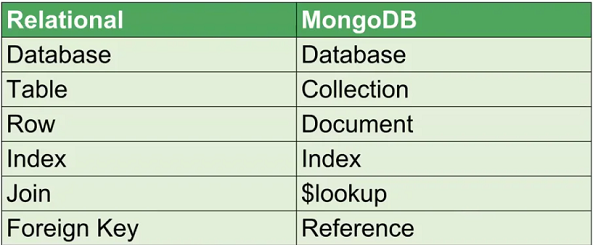
\includegraphics[scale=0.4]{Images/mongo2.png} 
    \label{mongo2_label}
    \caption{MongoDB vs relational DB}
\end{figure}

\subsection{MongoDB Atlas}
MongoDB Atlas is a cloud based system developed by MongoDB. Atlas provides an easy way to host and manage your data in the cloud with the service provider of your choice, for this application, I used Amazon Web Services (AWS).

Atlas uses clusters to manage the data in a MongoDB project. Clusters are simply Atlas-managed MongoDB deployments and can be either a replica-set or a sharded cluster \cite{Mongo:clusters}. (Figure ~\ref{mongo3_label}) shows my atlas project is a replica set with three nodes

\begin{figure}[h]
    \centering
    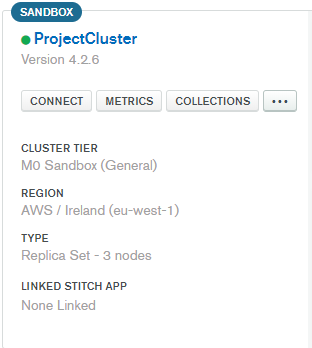
\includegraphics[scale=0.4]{Images/mongo3.png} 
    \label{mongo3_label}
    \caption{My MongoDB Project Cluster}
\end{figure}
A replica-set means there are multiple instances (in my case three) of MongoDB each mirroring all the data of the other. A replica-set consists of one primary node (master) and one or more secondary nodes (slaves). Read-operations can be served by any slave, but write-operations always take place on the master of the replica-set and are then propagated to the slaves. Replica-sets offer fault-tolerance as when one of the members of the replica-set goes down, the others take over. When the master goes down, the slaves will elect a new master.

\newpage
\subsubsection{Atlas In My Application}
To connect my Spring Boot application to my MongoDB cluster I simply had to configure it's connection address in the 'application.properties' file (Figure ~\ref{mongo5_label}).

\begin{figure}[ht]
    \centering
    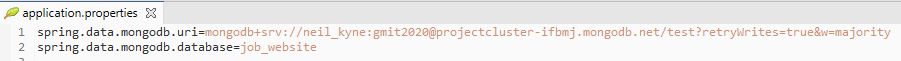
\includegraphics[scale=0.515]{Images/mongo5.png} 
    \label{mongo5_label}
    \caption{Connecting to My MongoDB Cluster}
\end{figure}
After providing the connection details above, our database, collection and all of the documents associated with that collection can be viewed on the MongoDB Atlas project page (Figure ~\ref{mongo1_label}).

\begin{figure}[ht]
    \centering
    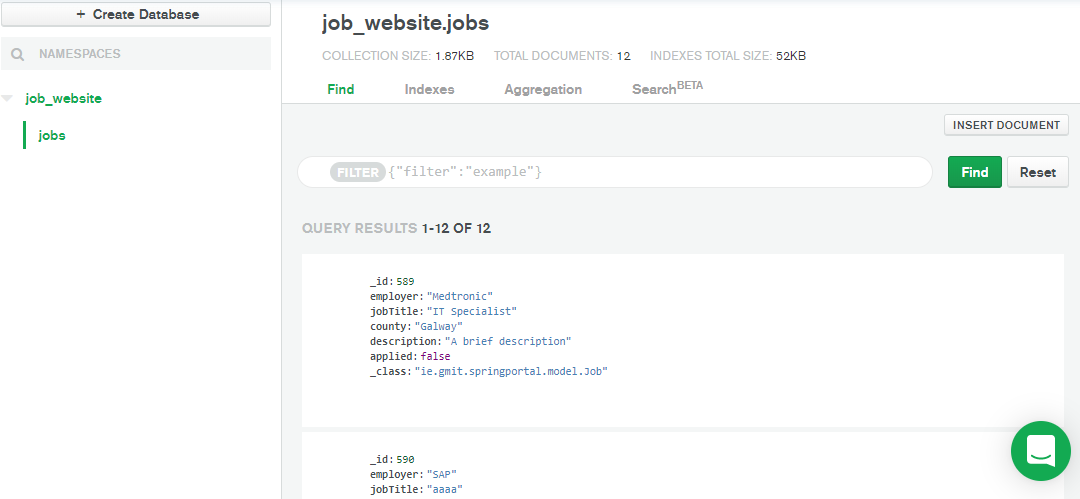
\includegraphics[scale=0.4]{Images/mongo1.png} 
    \label{mongo1_label}
    \caption{My MongoDB Database}
\end{figure}

\section{Spring Boot}
To properly understand Spring Boot we must first briefly summarize its foundation framework, Spring. Spring is one of the most popular Java Enterprise Edition (EE) Frameworks for building  web services. For the Java platform, the Spring framework provides an elaborate programming and configuration model. It can be used at any kind of deployment platform as unlike other frameworks, Spring focuses on several areas of an application and provides a wide range of features. However, in recent years, due to added functionalities, the Spring framework has become increasingly complex. It requires going through a lengthy procedure in order to start a new Spring project. To avoid starting from scratch and save time, Spring Boot has been introduced. This uses the Spring framework as a foundation \cite{DZone:Spring}.

Spring Boot allows developers to create stand-alone, production-grade Spring based Applications that you can "just run".
It take an opinionated view of the Spring platform and third-party libraries so you can get started with minimum fuss. Most Spring Boot applications need minimal Spring configuration \cite{Spring:SpringBoot}.

\subsection{Creating Spring Boot Application}
I chose to 'Bootstrap' my application with the 'Spring Initializr' provided on the official Spring website (Figure ~\ref{spring1_label}). This is a very handy tool that lets you pre-configure project settings such as dependencies, languages or project type (Maven) and get setup and ready to code within minutes.

\begin{figure}[ht]
    \centering
    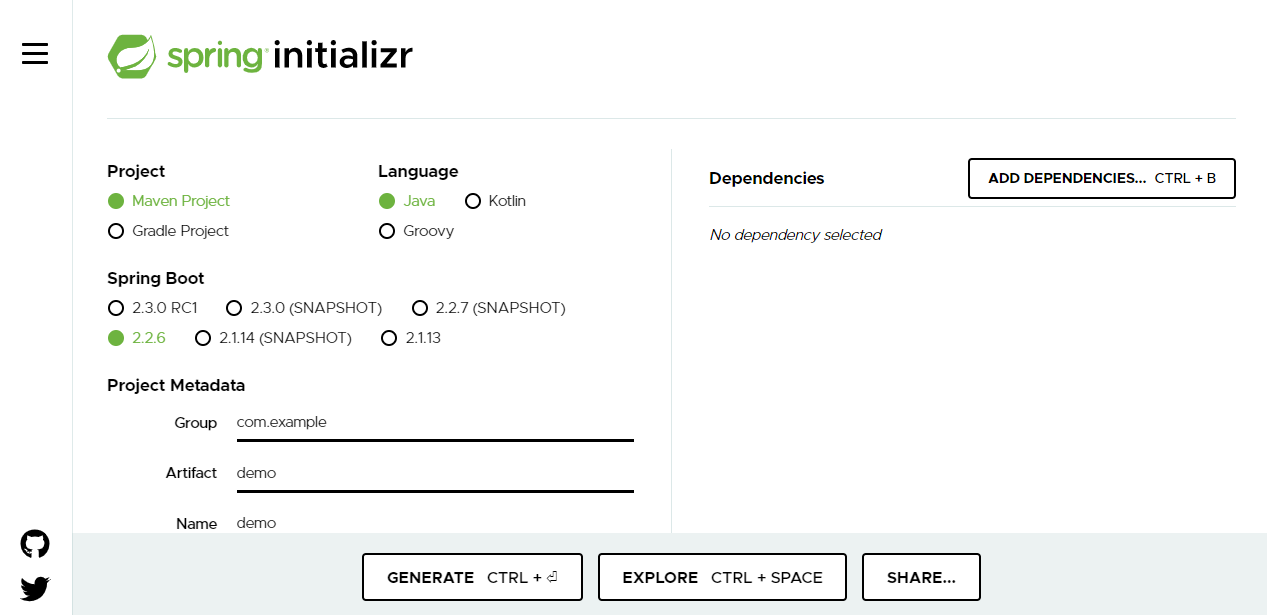
\includegraphics[scale=0.35]{Images/spring1.png} 
    \label{spring1_label}
    \caption{Spring Initializr Setup Page}
\end{figure}
Once I generated the Spring Boot project from the 'Initializr' I simply needed to import that package to Eclipse as a Maven project. As we can see in (Figure ~\ref{spring2_label}) all of the dependencies chosen in the Initializr have been added to the 'pom.xml' file.

\begin{figure}[ht]
    \centering
    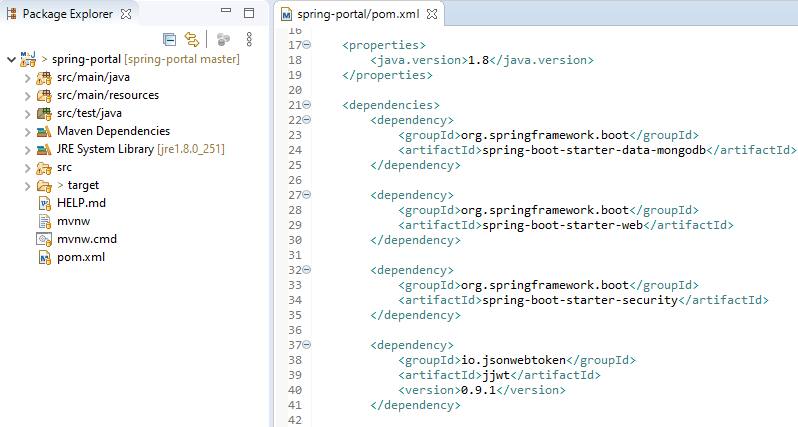
\includegraphics[scale=0.33]{Images/spring2.png} 
    \label{spring2_label}
    \caption{Spring Initializr Setup Page}
\end{figure}

\section{Heroku}
I mentioned earlier in the document I wanted my project to mimic what it would be like to develop a real website. Of course, my application can hardly hold a light to a user ready website we could find on the web at this moment, however, I did want it to be deployed in order to understand what is required to deploy a large application with multiple different technologies and tiers working together.

With this in mind, I decided to use Heroku as I had some experience with it from the module 'Software Engineering' already this semester.
Heroku is a container-based cloud Platform as a Service (PaaS). PaaS is a category of cloud computing that provides a platform allowing customers to develop, run, and manage applications without the complexity of building and maintaining the infrastructure typically associated with developing and launching an app \cite{wiki:paas}. Developers use Heroku to deploy, manage, and scale modern apps \cite{Heroku:about}.

To get my application fully hosted on Heroku I had to do three thing;
\subsubsection{1. Deploy my Spring Boot API}
In order for the front end to make calls to the API and display or manipulate job records on the web, I had to deploy the API as a separate Heroku application. I initially had no real problems with this until i deployed the React app and tried to make requests from the new address. I had forgotten to add the deployed application's front end address to the list of addresses permitted access to the API in the 'JobController' class as well as the 'JWTAuthenticationController' class (Figure ~\ref{heroku1_label}).

\begin{figure}[ht]
    \centering
    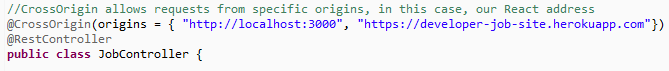
\includegraphics[scale=0.62]{Images/heroku1.png} 
    \label{heroku1_label}
    \caption{Permitting Cross Origin Requests}
\end{figure}

\subsubsection{2. Host my MongoDB Database on Atlas}
This was a relatively simple step and has mostly been covered already in the previous section on Atlas. I had to have my database in the cloud so it would be available to my API from anywhere at all times.
\subsubsection{3. Deploy my React App}
I created another Heroku application for the front end. This is the address that the user uses. As stated above, I had to add the front ends Heroku address to the Spring Boot controller classes in order to allow cross origin requests to the API (Figure ~\ref{heroku1_label}). Once I did this the application was fully deployed.

\section{React}
React (ReactJs) is a Javascript library for building user interfaces. React can be used as a base in the development of single-page or mobile applications. However, React is only concerned with rendering data to the Document Object Model (DOM), and so creating React applications usually requires the use of additional libraries for state management and routing \cite{React:wiki}. React Router is one such library I relied heavily upon for this application.

React uses a tool called 'Babel' to convert ES6 into a backwards compatible version of JavaScript that can be run by older JavaScript engines \cite{Babel}. ES6 is a more modern version of Javascript that brings useful features to a project such as the use of the 'let' and 'const' keywords, the spread operator or even arrow functions all of which are present in my application.

\subsection{Core Features}
Its most notable core feature, is the use of components and props. Components can be rendered to a particular element in the DOM using the React DOM library. When rendering a component, one can pass in values that are known as "props" \cite{React:components}. There are two types of components, 'functional components' and 'class components'. They differ in the fact that class components can hold 'state' values and can pass props to children (Figure ~\ref{react1_label}). Components are extremely useful as you can reuse them as many times as you need. They essentially return a section of the user interface. A well written 'Reactful' application would have lots of components each fulfilling its own purpose and nothing else. This makes an application maintainable.

\begin{figure}[h]
    \centering
    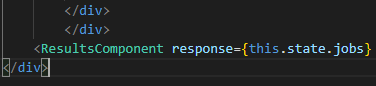
\includegraphics[scale=0.8]{Images/react1.png} 
    \label{react1_label}
    \caption{Passing a state value to 'ResultsComponent' as a prop called 'response'}
\end{figure}

Another notable features of React would be its use of 'Javascript-XML' (JSX). React uses JSX in place of HTML, it converts HTML tags into react elements. It is not required to use JSX in React although it is highly encouraged as it makes developing much easier. As demonstrated in (Figure ~\ref{react2_label}) the first line of code uses JSX, it lets us write HTML directly within a Javascript statement. Whereas in the second line, without the use of JSX, we must call the 'createElement' method and specify the tag. It's much easier to use JSX.

\begin{figure}[ht]
    \centering
    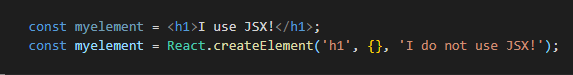
\includegraphics[scale=0.7]{Images/react2.png} 
    \label{react2_label}
    \caption{The same output, one with JSX and one without}
\end{figure}

\subsection{Creating React Application}
Like I did for creating my Spring Boot application, I made use of a very popular tool to help me speed up or 'bootstrap' the process of getting a React application off the ground. 'Create-React-App' is an official environment creator provided by the creators of React (Facebook) to help developers get set up to code within minutes. This powerful tool gets an application setup with the right set of dependencies such as babel, react-dom and ES6 without the developer ever having to worry.

To use 'Create-React-App' one must have Node and Node-Package-Manager (NPM) installed. Then they simply run 'npx create-react-app (application name)' and let their environment get setup.

Lastly, to run the react application in development mode we use the command 'npm start'. This runs the application on 'localhost:3000'.

\section{JSON Web Tokens}
As mentioned earlier, my application would need some form of authentication. For this, I used JSON Web Tokens (JWT). JWT is an open standard that defines a compact and self-contained way for securely transmitting information between parties as a JSON object. This information can be verified and trusted because it is digitally signed. JWTs can be signed using a secret or a public/private key pair \cite{JWT}, in regards to my application - a secret.

\begin{figure}[ht]
    \centering
    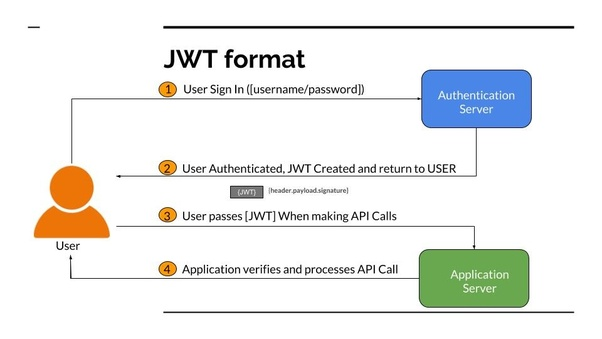
\includegraphics[scale=0.4]{Images/jwt1.jpeg} 
    \label{jwt1_label}
    \caption{JWT process}
\end{figure}

Specifically, JWT was used for authenticating and authorizing requests to and from my React application to my RESTful API. Below is a broad example of the steps that take place in my application when a user logs in:
\begin{itemize}
    \item The user sends a POST request to the '/authenticate' endpoint with a username and password. 
    \item The credentials are verified on the back end and a JWT is returned using a secret.
    \item The JWT and username are committed to the browser's session storage (not the password as it is sensitive data), this allows for verification on future requests.
    \item All subsequent API calls contain this JWT in their  authorization header using 'axios interceptors'.
    \item Application verifies whether or not the user is logged in (via session storage) and then processes the request.
\end{itemize}


\section{Secondary Technologies}
In this section I'll briefly analyze some of the secondary technologies and programs I used throughout the project that I found useful in development and think would be worthwhile mentioning.

\subsection{Postman}
Postman is a fantastic collaboration platform for API development. It makes it easy for developers to test and document their API as well as save requests in collections and share them with peers. Users can send basic HTTP requests or configure complex requests detailing a range of different authentication types, as well as read their responses. It also lets you send and receive data in a number of different formats such as XML, JSON or even HTML.

Postman is much more pleasant than using a browser and displays data really well. Below (Figure ~\ref{postman_label}) I have outlined some of the main components of my Postman environment:
\begin{enumerate}
    \item This area displays  the collections I created. Initially I just had one collection - 'Job API'. This grouped requests connecting to my locally hosted API, however after deploying the API to Heroku, I created a second collection for requests to that. Each collection groups requests into the 4 main HTTP request methods.
    \item This is where you enter the address and endpoint of the API you wish to connect to as well as the HTTP request method type.
    \item This is the request section. As shown below, I am making a POST request to the '/authenticate' endpoint, I'm passing it a username and password. If I was making a request to a different endpoint, I would include a JWT token in the 'Authorization' tab.
    \item This is the response section. As we can see, the server sent me back a JWT token. This area also shows the status of the request, in this case, '200 OK'. 
\end{enumerate}

\begin{figure}[ht]
    \centering
    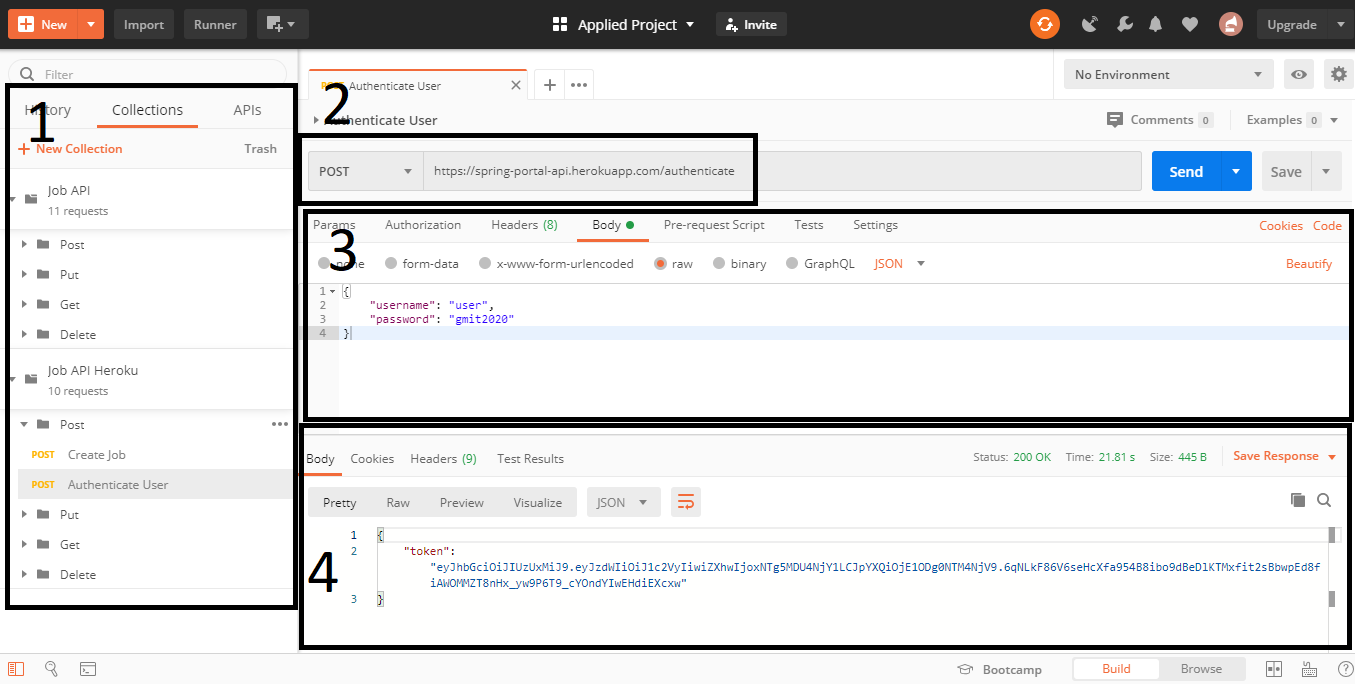
\includegraphics[scale=0.3]{Images/postman.png} 
    \label{postman_label}
    \caption{Postman home screen}
\end{figure}

\subsection{Jest \& React Testing Library}
For testing my React application I used two frameworks, \textbf{Jest} and \textbf{React Testing Library}.

\subsubsection{Jest}
Jest is a testing library developed by Facebook that can be used for regular Javascript applications as well as React applications. It comes pre-installed with React applications that are built using \textbf{Create-React-App}. In my application, to use Jest alone, no pre configuring was required.

\subsubsection{React Testing Library}
The React Testing Library makes it easy to test React components. \textbf{react-testing-library} runs tests that use actual DOM nodes rather than instances of React components. It also exposes a recommended way to find elements by a 'data-testid' (Figure ~\ref{testid_label}) as an "escape hatch" for elements where the text content and label do not make sense or is not practical \cite{TestingLibrary}.

\begin{figure}[h]
    \centering
    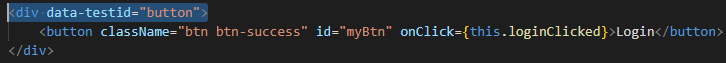
\includegraphics[scale=0.6]{Images/test1.png} 
    \label{testid_label}
    \caption{Identifying a button for testing using 'testid'}
\end{figure}

\subsection{GitHub}
As touched on in the Methodology chapter, GitHub was used throughout development to provide a back-up of my work and to document consistent progress over the seven or eight months I have been planning and developing the application. It's also very useful for version control and makes it easy to revert any changes to a project if a mistake is made via the commit history.

As I had mentioned, I regret not using more of GitHub's features to their fullest such as the Wiki or the Issues tracker. I did make some entries to the 'Issues' tracker late on in the project when I realised it would've been beneficial (Figure ~\ref{postman_label}). I documented my thoughts and progress mostly in Trello and a simple Word document but would've made better use of these features given a second run at the project.

\begin{figure}[ht]
    \centering
    \begin{minipage}{0.5\textwidth}
        \centering
        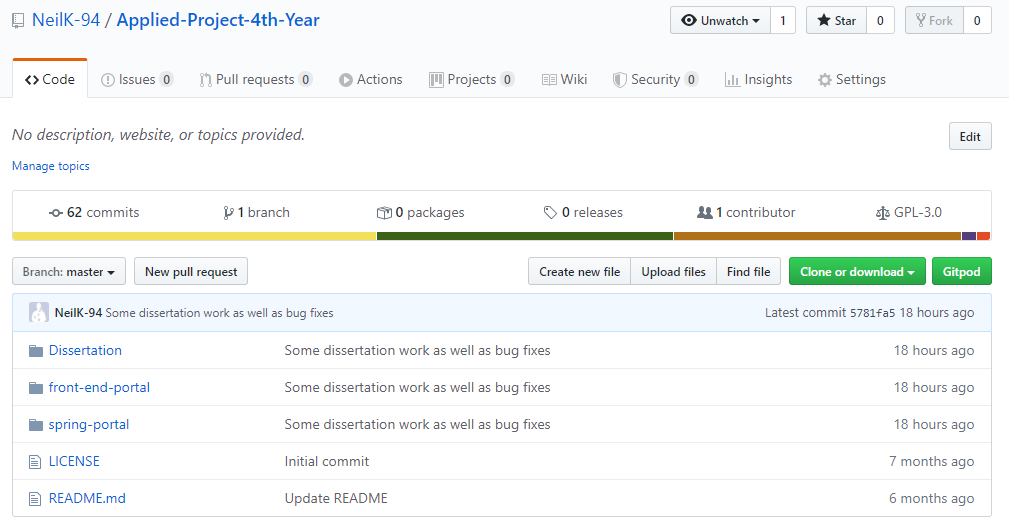
\includegraphics[scale=0.25]{Images/github1.png} 
        \label{git1_label}
        \caption{GitHub repository}
    \end{minipage}\hfill
    \begin{minipage}{0.5\textwidth}
        \centering
        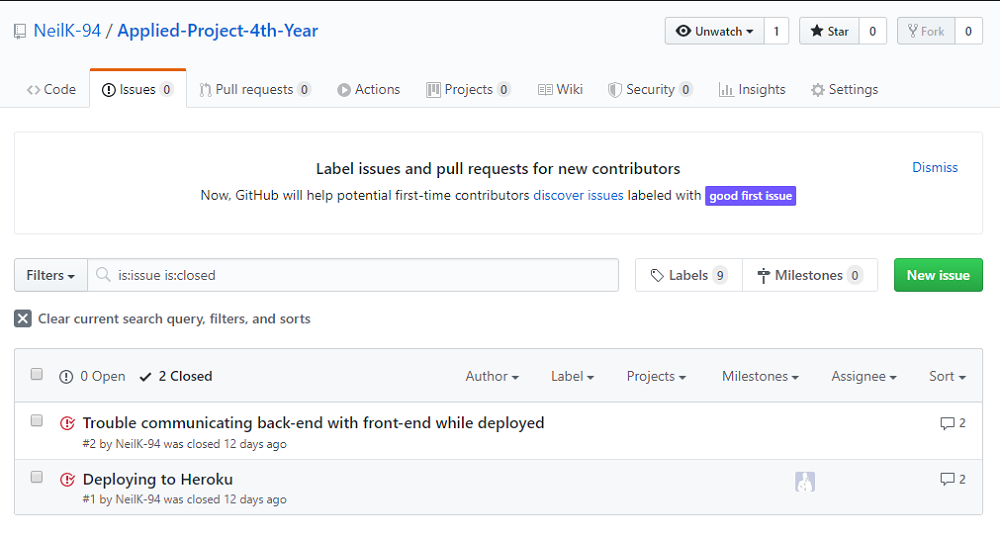
\includegraphics[scale=0.25]{Images/github2.png}
        \label{git2_label}
        \caption{GitHub issues tracker}
    \end{minipage}
\end{figure}

\subsection{React Frameworks}
Many different frameworks were used alongside the React library to develop the front end application, some of the most notable are the following:

\subsubsection{1. Bootstrap}
Bootstrap is an invaluable CSS framework which helps style web pages. I used it throughout my application and it is used to style almost every component. I initially imported the Bootstrap CSS via the site 'UNPKG'. This is a useful content delivery site for everything on NPM. I simply added the URL to a 'bootstrap.css' file and then imported it into my app (Figure ~\ref{boot_label}). Later on in development I added it via NPM also for easier use of features such as forms.

\begin{figure}[h]
    \centering
    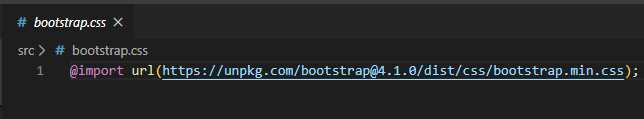
\includegraphics[scale=0.4]{Images/bootstrap1.png} 
    \label{boot_label}
    \caption{Bootstrap CSS file}
\end{figure}

\subsubsection{2. Axios}
Axios is a promise based HTTP client used to perform HTTP requests on API's. This framework was used for all requests coming and going from my front-end application.

\begin{figure}[h]
    \centering
    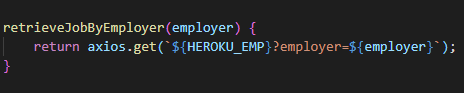
\includegraphics[scale=0.5]{Images/axios.png} 
    \label{axios_label}
    \caption{An Axios request}
\end{figure}

\subsubsection{3. React Router}
The React Router framework handles all the routing between components in my application. React Router is a widely used framework for React and can be found in most React applications. I used this framework extensively in my 'UserApp' component which acts as the central hub of my application. From here I control which web-pages are shown to the user (Figure ~\ref{router_label}), it is also used for authenticating all routes.

\begin{figure}[h]
    \centering
    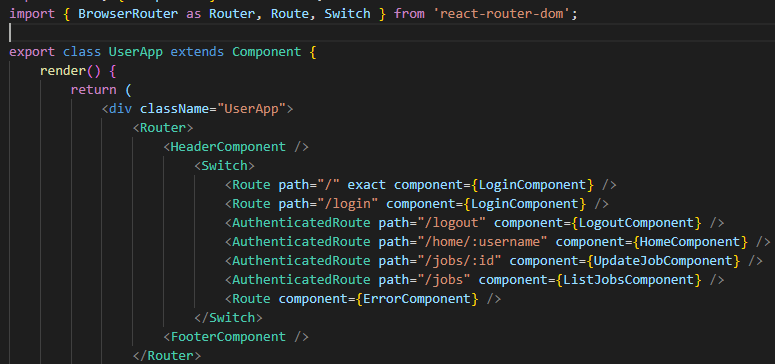
\includegraphics[scale=0.35]{Images/router.png} 
    \label{router_label}
    \caption{Main component using Router}
\end{figure}